\chapter{Recommender systems}

In a world of information overload, automatic filtering tools are essential to
extract relevant information from basic noise. In the field of e-commerce,
recommender systems play the role of search engines when surfing the entire
web: they filter available items to provide relevant suggestions to customers.

With the huge development of online businesses, recommender systems have become
more and more popular \cite{RecoSystemHandbook,AdoTuzIEEE2005}. They help to
answer questions as diverse as ``what movie to rent?", ``what item to buy?" or
``which restaurant to try?", but also such as ``what piece of code to
investigate ?" in the case of recommender system for software development.
They do so by providing the user with a list of recommendations.  Obviously,
the more personalized the recommendations, the better the system.  For
instance, a system recommending only the most popular items is useless as it is
likely that the standard customer knows these items. But the maximization of
business profit may also lead to suggest items which are not very popular (and
thus difficult to sell), provided they may be of interest for the user.

A very common way of providing personalized recommendations to a target user is
to estimate its taste for the items that the system provides. The taste of a user
$u$ for a given item $i$ is usually represented as a rating that $u$ would give
to $i$.  The scale of the ratings may vary, but the integer interval [1, 5] and
the \textit{like}/\textit{dislike} scales are very common in real world
systems.

Once these estimations are made, a simple option is to recommend the items with
the highest ratings among all the estimated scores for the considered user
(using the implicit assumption that a user should be interested in the items
with high scores).

Providing an accurate measure of the overall quality of a recommender system is
not a simple task and diverse viewpoints have to be considered (see
\cite{RecoSystemHandbook} for an extensive survey).  Obviously, accuracy of
its core prediction algorithm is an important matter, but other properties are
also desirable in order  to deploy an effective recommendation engine. For
instance {\it coverage} measuring what is the range of items in the catalogue
that could be recommended, or {\it serendipity} measuring in some sense the
surprise that a user could get when a new item is suggested.

\section{Background on recommender systems}
\label{sec:background_RS}

The aim of a recommendation system is to provide users with lists of relevant
personalized items.  Let us now formalize the problem.

\subsection{Problem formalization and notation}
Let $U$ be a set of users and $I$ a set of items. For some pairs $(u,i) \in U
\times I$, a rating  $\rui$ is supposed to have been given by $u$ to express
whether she likes the item $i$ or not.  It is quite common that  $\rui$ belongs
to the rating scale $[1, 5]$, 5 meaning a strong preference for item $i$, 1
meaning a strong rejection, and 3 meaning indifference, or just an average
note. When the rating scale is gradually valuated, we say that ratings are
\textbf{explicit}, in the sense that users have explicitely expressed their
preference towards items. \textbf{Implicit} ratings belong to a binary scale $[0,
1]$, and usually correspond to the result of collected data about users
behaviour, without any active involvement. For example, if a user has listened to a given track more than 10
times, we might consider this as an implicit rating of $1$. We may also
consider that an implicit rating captures the fact that a user has bought a
given item without giving it an explicit rating. These two kinfs of rating
schemes (explicit and implicit) lead to quite different prediction algorithms
in practice. In our work, we will only focus on the explicit rating
scheme.\todo{Vrai?}

Let us denote by $R$ the set of known ratings recorded in the system. It is
well known that, in real systems, the size of $R$ is very small with regard to
the potential number of ratings which is $|U| \times |I|$, as a lot of ratings
are missing. The set $\Ui$ will denote the set of users that have rated item
$i$, and $\Uij$ is the set of users that have rated both item $i$ and item $j$.
Similarly, $\Iu$ is the set of items that user $u$ has rated, and $\Iuv$ is the
set of items that both users $u$ and $v$ have rated.

To recommend items to users, a recommender system usually proceed as follows:
\begin{enumerate}
\item Using a prediction algorithm $A$, estimate the unknown ratings $\rui$
  (i.e. $\rui \notin R$). This estimation $A(u, i)$ will here be denoted
    $\predrui$.
\item Using a recommendation strategy $S$ and in the light of the previously
  estimated ratings, recommend items to users. For instance, a basic yet common
    strategy is to suggest to user $u$ the items $i \notin I_u$ with the
    highest $\predrui$.
\end{enumerate}

When using the implicit rating scheme, these two stages are usually
indistinguishable: it is natural to recommend an item to a user if the
estimated predicted rating is $1$. In practice, the recommendation strategy
depends a lot on the pragmatic constraints of the system: a store manager way
want to push forward a given item to boost its sellings, regardless of the
rating predictions outputted by the algorithm. As a result, most of the
research has focused on the prediction algorithms, and so will we.

Prediction algorithms implementations are strongly influenced by the fields of
data mining and of course machine learning. However, we want to emphasize that
the general setting of recommender systems is actually quite different than
that of classification or regression. A naïve reasoning could lead us to
consider that the rating prediction problem with the rating scale $[1, 5]$ is
nothing but a classification task with five classes $1, 2, 3, 4, 5$. But this is
forgetting that the values $1, 2, 3, 4, 5$ are actually ordinal, and that the
difference between \textit{class} $1$ and \textit{class} $2$ is not the same as the
difference between \textit{class} $1$ and \textit{class} $4$. But most
importantly, in classification or regression all the instances belong to the
same space (that space was $X^m$ in our previous chapters), and have the same
features. This is not the case here! In a recommendation problem, if we chose
our instances to be the users and their feature space to be the items, we would
end up with instances that are only (very) partially described, because of
course no user has rated the whole set of items. All the more, as the number of
items is usually very high, we would end up with a very high dimensional
problem, where learning algorithm tend to fail due to the so-called curse of
dimentionality. Our point here is that recommender systems problems do not
really fit within the traditional machine learning setting, and represent a new
setting in their own right.

Traditionally, prediction algorithms are
considered to belong to one of the two main families of prediction techniques,
referred to as \textbf{content-based} methods and \textbf{collaborative
filtering} methods, that we both review below. In practice, real-world
recommender systems usually use a mix of both methods, and are referred to as
\textbf{hybrid} methods.

\subsection{Content-based techniques}
\label{SEC:collaborative_filtering}

Content-based algorithms try to recommender to a user some items that are
\textbf{similar} to those that the user has liked in the past. For example, if
the renting history of a user mainly contains science fiction movies, the aim
of the system is to learn these preferences and recommend some other science
fiction movies to the user. We recommend \cite[Ch.~3]{RecoSystemHandbook} for a
recent overview of content-based methods.

To find out similar items to those that a user has liked, these systems usually
rely on a similarity metric whose nature strongly depends on the representation
of the items. In large-scale online shopping systems were items are extremely
diverse and abundant, a similarity measure between two items would be for
example the number of web sessions on which the two item pages have jointly
been visisted (yes, this is the reason why some online systems will try to sell
you a fridge even though you just bought a brand new one). In systems were
items are more homogeneous, i.e. in a movie store system, more  sophisticated
approaches can be built relying on some metadata about the items (hence the
name \textit{contenat}-based), for example movies genre, main actors, film
director, etc\dots.

As content-based techniques do not rely on the set of ratings to compute item
similarities, a nice resulting feature is that new items that have not yet been
rated by anybody can still be recommended. Content-based techniques also stand
out by their explanatory potential: the motto \textit{Here are some items that
are akin to those you liked} is perfectly understandable and seems sound.
Recommender systems usually strive for explanatory power, because it is
recognized that when confronted with a given recommendation users are more
likely to accept the recommendation is they understand and acknowledge the
underlying process.

However, content-based systems are prone to various behaviour that tend to make
them less competitive with other collaborative filtering methods. The first
obvious drawback is that most of the time, metadata are required to describe
the items (remember our movie example with genre, actors etc.). Such
description can be extremely costly and can only capture a very limited subset
of item features, which are not necessarily the most important ones when it
comes to the users personal tastes. Going back to our science fiction fan, it
is very plausible that the user has a strong preference for the steampunk
genre, and yet is perfectly indifferent to the superhero fiction movies, and
both can still be considered as subgenres of science fiction. A system that
could not distinguish these two kinds of movies would fail to provide our
steampunk fan with relevant recommendations.

Another well-known drawback of content-based recommenders is their tendency to
recommend only items that users may already know or do not need anymore (such
as a fridge!), and therefore the recommendations lack in novelty, surprise and
diversity. Also, they tend to output much less accurate prediction the
collaborative filtering methods (the way accuracy is computed will be described
in Section \ref{TODO}). For all these reasons, our own analogy-based algorithms
we rather be of a collaborative filtering nature.

\subsection{Collaborative filtering techniques}
\label{SEC:collaborative_filtering}

The main idea behind collaborative filtering algorithms is to recommend items
to a users that other users with similar tastes have liked in the past. So for
example if Bob and Alice usually agree on their movie ratings, i.e. they like
the same movies and dislike the same movies, if Alice has not seen a movie that
Bob has liked, then it will be recommended to Alice. We will here present two
families of collaborative filtering algorithms: the neighborhood approach based
on the well known $k$-NN algorithm, and the matrix factorization techniques
whose groundings come from linear algebra and that lead to elegant and accurate
models.

\subsubsection{The neighborhood approach}

Neighborhood approaches are instances of the general $k$-NN scheme. To estimate
the rating $\rui$ of a user $u$ for an item $i$, the most basic method consists
in computing  the set of $k$ users that are most similar to $u$ and
that have rated $i$. We will denote this set $N_i^k(u)$. The computation of
$N_i^k(u)$ depends of course on a similarity measure between users, which is
based on their respective ratings.  The estimation $\predrui$ of $\rui$ is then
computed as an aggregate of the ratings $\rvi$, where $v$ is one of the
neighbors of $u$. Usually, the aggregation is simply a mean weighted by the
similarity between $u$ and $v$: $$\predrui = \frac{\sum\limits_{v \in N_i^k(u)}
r_{vi} \cdot \ssim(u, v)} {\sum\limits_{v \in N_i^k(u)}\ssim(u, v)}.$$

There are many, many ways to define the similarity metric between two users.
Probably the most common one is the cosine similarity:
$$
\text{cosine sim}(u, v) = \frac{ \sum\limits_{i \in \Iuv} \rui \cdot \rvi}
{\sqrt{\sum\limits_{i \in \Iuv} \rui^2} \cdot \sqrt{\sum\limits_{i \in \Iuv}
\rvi^2}}.
$$

Here, users $u$ and $v$ are considered as vectors in a vector space defined by
the items they have both rated. Their cosine similarity simply is the cosine of
the angle between the two vectors. An unnatural feature of this metric is that
two vectors with (potentially different) constant values will always have a
similarity of $1$, because they are collinear. For example if $u = (2, 2)$ and
$v = (5, 5)$, $\text{cosine sim}(u, v) = \frac{20}{\sqrt{8}\sqrt{50}} = 1$,
while one would expect $u$ and $v$ to be quite different w.r.t. their tastes.

Such a flaw can be overcame using the Pearson similarity, which can be viwed as
a mean-centered version of the cosine similarity:

$$
\text{pearson sim}(u, v) = \frac{ \sum\limits_{i \in \Iuv}
(\rui -  \mu_u) \cdot (\rvi - \mu_{v})} {\sqrt{\sum\limits_{i
\in \Iuv} (\rui -  \mu_u)^2} \cdot \sqrt{\sum\limits_{i \in
\Iuv} (\rvi -  \mu_{v})^2}},
$$
where $\mu_u$ and $\mu_v$ are the average rating of users $u$ and $v$
respectively.

One last similarity metric that we will use is the Mean Squared Difference
(MSD)\footnote{Strictly speaking MSD is actually a distance rather than a
similarity metric, so taking its inverse would do the job.}:
$$\text{MSD}(u, v) = \frac{1}{|\Iuv|} \cdot \sum\limits_{i \in \Iuv} (\rui -
\rvi)^2$$

In the next section, we describe another very popular collaborative filtering
technique, which models the data in a significantly different (but meaningful!)
way.

\subsubsection{Matrix factorization techniques}

About ten years ago, the Netflix company organized a competition where the goal
was to outperform the RMSE (defined in Section \ref{TODO}) of their standard
prediction algorithm of $10\%$. The challenge quickly became very popular, not
only because the winning prize was of \$1 million, but also because the dataset
was orders of magnitude bigger than any other available dataset so far: about
100M of ratings of 480.000 user sand 17.700 movies. Unfortunately, their
dataset is no longer publicly available, but the challenge led to the emergence
of many successful recommendation technique, among which matrix factorization
methods clearly stand out.

The matrix factorization approach we will describe here is heavily inspired by
the Singular Value Decomposition (SVD) of a matrix, one of the highlights of
linear algebra. Because having a basic understanding of SVD will be very
insightful for us, we will try to briefly describe it here. Let's first dive
into the arid theory (not for long):

\begin{proposition}
  Any real-valued matrix $R \in \mathcal{M}^{m \times n}$ of rank $r$ can be
  decomposed as the product of three matrices:

  $$R = P\Sigma Q^t,$$
  where $P\in \mathcal{M}^{m \times r}$, $\Sigma\in \mathcal{M}^{r \times r}$
  is a diagonal matrix, and $Q\in \mathcal{M}^{n \times r}$.
\end{proposition}

As $\Sigma$ is a diagonal matrix, it only act as a scaler for either $P$ or
$Q$. For the sake of simplicity, we will consider that the decomposition can be
written $R = PQ$, where $\Sigma$ has been merged into either $P$ or $Q$. In
practice, we know how to compute the columns of $P$ and $Q$: they are the
eigenvectors\footnote{For this reason, SVD and Principal Component Analysis are
strongly related.} of the two matrices $A^tA$ and $AA^t$, and their associated
eigenvalues are the squared entries of $\Sigma$, called the singular values
(hence the name of the factorization).

The key point is that the columns of $P$ are actually an orthonormal basis for
the column space of $R$, and columns of $Q$ are an orthonormal basis for the
row space of $R$. Maybe this statement is worth some explaination. The column
space of $R$ is the vector space that is spanned by the $n$ columns or $R$,
i.e. the set of vectors that are a linear combination of the columns of $R$. As
some of the columns of $R$ may be linearly dependent, this vector space is of
dimension $r\leq n$: the rank of a matrix is defined as the number of
independent columns, and equivalently as the number of independent rows. Our
statement says that the columns of $P$ span the same space, and that they form
an orthonormal basis of $r$ vectors. The same goes the columns of $Q$, which
span the row space of $R$.

A particular case of this general statement is that \textbf{any column of $R$
can be expressed as a unique linear combination of the columns of $P$}. As the
columns of $P$ are orthonormal, each column has a unique contribution that
cannot be compensated by the others. Symmetrically, \textbf{any row of $R$ is a
linear combination of the columns of $Q$.} What does it have to do with our
recommendation problem? Imagine for a moment that $R$ is a dense rating matrix,
where the rows reprensent items and the columns reprensent users:
$$
R = \begin{blockarray}{cccc}
  \text{Alice} & \text{Bob} & \text{Charlie} \\
\begin{block}{(ccc) c}
  4 & 5 & 5 & \text{Titanic} \\
  2 & 1 & 1 & \text{Toy Story} \\
  1 & 2 & 2 & \text{LORT} \\
  3 & 3 & 3 & \text{Mad Max} \\
  4 & 2 & 2 & \text{E.T.} \\
\end{block}
\end{blockarray}
=
\begin{pmatrix}
  \\
  p_1& p_2 & \cdots & p_r\\
  \\
\end{pmatrix}
\begin{pmatrix}
  & q_1 & \\
  & q_2 & \\
  & \vdots & \\
  & q_r & \\
\end{pmatrix}
$$




If we perform the SVD of $R$, we will find in the columns of $P$ some
\textit{prototype} users that have no real existence, but that can be combined
(linearly) to build up either Alice, Bob or Charlie. Similarly, the columns of
$Q$ are \textit{prototype} movies that do not properly exist but that can be
combined to build up Titanic, Toy Story, etc\dots

it postulates the existence of $f$
factors/criteria
(whose nature is not necessarily known) that determine the value of any rating
$\rui$.  A user $u$ is modeled as a vector $p_u \in \mathbb{R}^f$, where each
component of $p_u$ models the importance of the corresponding factor for $u$.
Similarly, an item $i$ is modeled as a vector $q_i \in \mathbb{R}^f$, where
each component of $q_i$ models how well $i$ fits the corresponding criteria.
From then, a rating prediction $\predrui$ is calculated as the dot product
of the two vectors $p_u$ and $q_i$: $$\predrui = p_u^t \cdot q_i$$. 

Once the number of factors is set, the problem is here to estimate the vectors
$p_u$ and $q_i$ for every possible users and items. This can be done by solving
the following regularized least square optimization problem:
$$
\sum_{\rui \in \Rtrain} \left(\rui - q_i^t \cdot p_u \right)^2 +
\lambda\left(\norm{}{q_i}^2 + \norm{}{p_u}^2\right),
$$
where $\lambda$ is a regularization term. Not surprisingly, stochastic gradient
descent tend to perform really well on this task, but Alternating Least Squares
can also be used.

\todo{Mettre des refs}

Contrary to the neighbourhood-based approach, the matrix factorization
technique tends to model global aspects of the data.  Matrix factorization and
neighbourhood based techniques have been successfully mixed in the works of
\cite{KorACM2010}.

\subsection{Recommender system
evaluation}\label{eval} Providing an accurate measure of the overall quality of
a recommender system is not a simple task and diverse viewpoints have to be
considered (see \cite{RecoSystemHandbook} for an extensive survey).
% Obviously
%accuracy is an important matter as  any system includes a prediction algorithm,
%but other properties are also desirable in order  to deploy an effective
%recommendation engine.

\paragraph{Accuracy\\}
The performance of the algorithm $A$ is usually evaluated in terms of accuracy,
which measures how close the rating prediction $\predrui$ is to the true
rating value $\rui$, for every possible prediction. To evaluate the accuracy
of a prediction algorithm, one usually follows the classical machine learning
framework: the set of ratings $R$ is divided into two disjoint sets $\Rtrain$
and $\Rtest$, and the algorithm $A$ has to predict ratings in $\Rtest$
based on the ones belonging to $\Rtrain$.

The Root Mean Squared Error (RMSE) is probably the most common indicator of
how accurate an algorithm is, and is calculated as follows:
$$\text{RMSE}(A) = \sqrt{\frac{1}{|\Rtest|} \cdot \sum_{\rui \in
\Rtest}(\predrui - \rui)^2}.$$

Another common indicator for accuracy is the Mean Absolute Error (MAE), where
important errors are not penalized more than small ones:
$$\text{MAE}(A) = \frac{1}{|\Rtest|} \cdot \sum_{\rui \in \Rtest}|\predrui -
\rui|.$$

In order to have reliable estimates of the accuracy measures, $k$-folds
cross-validation procedures are often used: the set of all ratings $R$ is
divided into $k$ disjoint sets ; at each of the $k$ iterations, $\Rtrain$ is set
to the $k^{\text{th}}$ subset and $\Rtest$ is set as the $k - 1$ remaining
ones. The reported RMSE (or MAE) is then the average of the $k$ measures.

To better reflect the user-system interaction, other precision-oriented metrics
are sometimes used in order to provide a more informed view.
\todo{Mieux parler des critiques faites à RMSE et MAE}

\paragraph{Precision and recall\\}
Precision and recall help measuring the ability of a system to provide
relevant recommendations.
In the following, we denote by $I_{S}$ the set of items that the strategy
$S$ will suggest to the users using the predictions coming from $A$. For
ratings in the interval $[1, 5]$, a simple strategy could be for example to
recommend an item $i$ to user $u$ if the estimation rating $\predrui$ is
greater than $4$.  $$I_S = \{i \in I | \exists u \in U, \predrui \geq
4\}.$$

Let $I_{relev}$ be the set of items that are actually relevant to users (i.e.
the set of items that would have been recommended to users if all the
predictions made by $A$ were exact).
The precision of the system is defined as the fraction of recommended items that
are relevant to the users:
$$\text{Precision} = \frac{|I_{S} \cap I_{relev}|}{|I_{S}|},$$
and the recall as the fraction of recommended items that are relevant to the
users out of all possible relevant items:
$$\text{Recall} = \frac{|I_{S} \cap I_{relev}|}{|I_{relev}|},$$

If accurate predictions are crucial, it is widely agreed that it is
insufficient for deploying an effective recommendation engine. Indeed, still
other dimensions are worth estimating in order to get a complete picture of the
performance of a system
\cite{NeeRieKonACM2006,HerKonJohTerRieACM2004,KamBriRecSys2014}.
For instance, one may naturally expect from a recommender system
not only to be accurate, but also to be surprising, and to be able to recommend
a large number of items. When evaluating the recommendation strategy, one must
keep in mind that its performance is closely related to that of the algorithm
$A$, as the recommendation strategy $S$ is based on the predictions provided by
$A$.


\paragraph{Coverage\\}
Coverage, in its simplest form, is used to measure the ability of a system to
recommend a large amount of items: it is quite easy indeed to create a
recommender system that would only recommend very popular items. Such a
recommender system would drop to zero added value. Coverage can be defined as the
proportion of recommended items out of all existing items:
$$\text{Coverage} = \frac{|I_{S}|}{|I|}.$$



\paragraph{Surprise\\}
Users expect a recommender system to be surprising: recommending an extremely
popular item is not really helpful. Following the works of
\cite{KamBriRecSys2014}, surprise of a recommendation can be evaluated with the
help of the pointwise mutual
information (PMI). The PMI between two items $i$ and $j$ is defined as follows:
$$PMI(i, j) = -\log_2 \frac{p(i, j)}{p(i)p(j)} / \log_2 p(i, j),$$
where $p(i)$ and $p(j)$  represent the probabilities for the items to be rated
by any user, and $p(i, j)$ is the probability for $i$ and $j$ to be rated
together: $p(i) = \tfrac{|U_i|}{|U|}$ and $p(i, j) = \tfrac{|U_i \cup
U_j|}{|U|}$. PMI values fluctuate between the interval $[-1, 1]$, $-1$ meaning
that $i$ and $j$ are never rated together and $1$ meaning that they are always
rated together. To estimate the surprise of recommending an item $i$ to a user
$u$ we have two choices:
\begin{itemize}
\item either to take the maximum of the PMI values for $i$ and all
other items rated by $u$, with $Surp^{max}(u, i) = \max\limits_{j\in I_u} PMI(i, j)$
\item
 or to take the mean of these PMI values with $Surp^{avg}(u, i) =
\frac{\sum_{j \in I_u} PMI(i, j)}{|I_u|}$
\end{itemize}
Then the overall capacity of a recommender to surprise its users is the mean of the
surprise values for all predictions.

\section{Analogical recommendation}
\label{sec:analogical_recommendation}

The main idea is that if an analogical proportion stands between four
users $a, b, c, d$, meaning that for each item $j$ that they have commonly
rated, the analogical proportion $r_{aj} : r_{bj} :: r_{cj} : r_{dj}$ holds,
then it should also hold for an item $i$ that $a, b, c$ have rated but $d$ has
not (i.e. $r_{di}$ is the missing component). This leads us to estimate
$r_{di}$ as the solution $x = \hat{r}_{di}$ of the following analogical equation:
$$r_{ai} : r_{bi} :: r_{ci} : x.$$
\noindent
Given a pair $(u,i)$ such that $r_{ui} \notin R$, the main procedure is as
follows:
\begin{enumerate}
\item find the set of 3-tuples of users $a, b, c$ such that an analogical proportion
stands between $a, b, c,$ and $u$ and such that the equation $r_{ai} : r_{bi} :: r_{ci} : x$
is solvable.
\item solve the equation $r_{ai} : r_{bi} :: r_{ci} : x$ and consider the solution
$x$ as a candidate rating for $r_{ui}$.
\item set $\hat{r}_{ui}$ as an aggregate of all candidate ratings.
\end{enumerate}

\subsection{An algorithm using arithmetic proportion}
In the following, let $I_{abcu}$ be the set of items $i$ that users $a, b, c,$
and $u$ have commonly rated: $r_{ai} \in R, r_{bi} \in R, r_{ci} \in R$ and
$r_{ui}\in R$.
The first step simply states that users $a, b, c$ and $u$, considered as
vectors of ratings, constitute a parallelogram.  This condition is a bit strong
and we may want to relax it by allowing some deformation of this parallelogram.
This can be done by choosing another condition, such as $||(a-b) - (c-d)|| \leq
\lambda$ where $\lambda$ is a suitable threshold and $||.||$ denotes the
Euclidean norm.

Another modification to the algorithm would be to only search for the users
$a, b,$ and $c$ in a subset of $U$. One may consider the set of the $k$-nearest
neighbours of $d$, using the assumption that neighbours are the most relevant
users to estimate a recommendation for $d$.

Obviously, analogical proportion may be applied in an item-based way rather
than in a user-based way, as in the case of standard techniques. Both views
will be considered in the experimentation.

\subsubsection{Implementation}

In our implementation, we consider the basic definition of analogy using the
arithmetic definition in $\mathbb{R}^n$: $\vec{a}:\vec{b}::\vec{c}:\vec{d}
\iff \vec{a}-\vec{b}=\vec{c}-\vec{d}$.
Given 4 users, they are represented as real vectors of dimension $m$, where $m$
is the number of item they have rated in common. This dimension can
change with the 4-tuples of users that we consider.
Then, the threshold $\lambda$ has to be a function of this dimension $m$,
as the range of values that $||.||$ may take depends on it. Using
cross-validation, we have found that $\lambda = \frac{3}{2} \cdot\sqrt{m}$ showed the
best results and acts as a kind of normalization factor.
Our pseudo-code is described in
Algorithm \ref{algo:analogical_reco}.
 \begin{algorithm}[!ht]
       \begin{algorithmic}

      \STATE {\bf Input}: A set of known ratings $R$, a user $u$, an item
      $i$ such that $r_{ui} \notin R$.
      \STATE {\bf Output}: $\hat{r}_{ui}$, an estimation of $r_{ui}$

      \STATE {\bf Init}:
      \STATE $C = \varnothing$ \quad \quad // list of candidate ratings
      \FORALL{
        users $a, b, c$ such that\\
        \begin{enumerate}
        \item $r_{ai} \in R, r_{bi} \in R, r_{ci} \in R$
        \item $r_{ai} - r_{bi} = r_{ci} - x$ is solvable  // i.e. the solution $x \in [1,5]$
        \item $||(a-b)-(c-d)||\leq \lambda$ // Analogy almost stands between $a,b,c,d$ considered as real vectors
        \end{enumerate}
      }

      \STATE  $x \leftarrow r_{ci} - r_{ai} + r_{bi}$
      \STATE $C \gets C \cup \{x\}$ \quad // add x as a candidate rating
	  \ENDFOR

    \STATE $\hat{r}_{ui} = \aggr{x \in C} x$

\end{algorithmic}
     \caption{Analogy}
       \label{algo:analogical_reco}
\end{algorithm}

Some options are available at this stage.

Here again, there is no need to choose the Euclidean norm (i.e. $L_2$ norm) as
other norms also make sense: $L_1$ norm using the absolute value of the
components or even $L_\infty$ using the maximum of the absolute value of the
components. These options have not been tested so far.

We have considered a strict condition for the solvability of the equation
$r_{ai} - r_{bi} = r_{ci} - x$: as the exact arithmetic result $x=r_{ci} +
r_{bi} -r_{ai}$ does not necessarily belong to the scale interval $[1,5]$, we
consider solvability only when $r_{ai}=r_{bi}$ or $r_{ai}=r_{ci}$. In both
cases, we ensure the solution $x \in [1,5]$.

\subsection{Experiments and results}
\label{results}

Our algorithm \textit{Analogy} ($k=20$) is compared to the neighbourhood-based algorithms
described in section \ref{CollabFil}, referred to as \textit{kNN} for the basic
model and \textit{Bsln-kNN} for the extended model using a baseline predictor
(with $k=40$). For each of the algorithms, we have estimated the metrics described
in section \ref{eval}. The recommendation strategy $S$ is to recommend $i$ to
$u$ if $\hat{r}_{ui} \geq 4$.

\paragraph{Dataset\\}
We have tested and compared our algorithm on the Movielens-100K
dataset\footnote{http://grouplens.org/datasets/movielens/}, composed of 100,000
ratings from 1000 users on 1700 movies. Each rating belongs to the interval
$[1, 5]$.

\paragraph{Evaluation protocol\\}
In order to obtain meaningful measures, we have run a five-folds
cross-validation procedure: for each of the five steps, the set of ratings $R$ is
split into two disjoint sets $R_{train}$ and $R_{test}$, $R_{train}$ containing
five times more ratings than $R_{test}$. The reported measures are averaged
over the five steps.

\paragraph{Results and comments\\}

Table \ref{table:res} shows the performances of the algorithms applied in a
user-based way. Similar experiments have been led in a movie-based setting, exhibiting
very similar results, slightly worse for RMSE (about 5\permil higher).

\begin{table}[ht]
\begin{tabular}{| c || c | c | c | c | c | c | c | c |}
\hline
& RMSE & Prec & Rec & Cov & $Surp^{max}$ & $Surp^{avg}$ & Time \\
\hline
Analogy   & .898 & 89.1 & 43.3 & 31.2 & 0.433 & 0.199 & 2h \\
%Pattern & .927 & 84.9 & 50.0 & 47.7 & 0.433 & 0.198 & 5h \\
kNN     & .894 & 89.1 & 44.1 & 27.8 & 0.432 & 0.198 & 10s \\
Bsln-kNN & .865 & 88.4 & 44.0 & 44.7 & 0.431 & 0.199 & 10s \\
\hline
\end{tabular}

\caption{Performance of algorithms}
  \label{Zob}
\end{table}

As expected, the Bsln-kNN algorithm is more accurate than the basic
collaborative filtering method (KNN). The two classical collaborative
algorithms perform better than the new proposed analogy-based method in terms
of RMSE. Still, there seems to be some room for improvement for the analogical
approach, with the help of a careful analysis of the behaviour of the
algorithm.

As for performances other than RMSE, we see that the figures obtained by the
three algorithms are quite close. Regarding surprise, which is a delicate
notion to grasp, one may also wonder if the used measure is fully appropriate.

As usual, analogy-based algorithms suffer from their inherent cubic complexity.
In the case of recommender systems where millions of users/items are involved,
this is also a serious issue.

\section{Clones}

Considering analogy between four users has shown to be computationally
intensive, thus not really suitable for recommendation purposes, where time is
a highly critical dimension. Yet, other forms of analogy can be addressed in
the recommendation task, based on the observation that some users may be more
inclined to give good (or bad) ratings than others. Indeed, ratings are in no
way absolute and greatly depend on the subjective appreciation each user has
about the rating scale. In the $[1, 5]$ scale for example, two users $u$ and
$v$ might semantically agree on an item $i$ describing it as $bad$, but there
is a chance that this agreement is not perfectly reflected in the ratings: $u$
might have rated $i$ with $r_{ui} = 1$ and $v$ with $r_{vi} = 3$, simply
because from $v$' point of view $3$ is a \textit{bad} rating, while for $u$ a
rating of $3$ would simply mean \textit{decent} or \textit{good enough}.  In
the following, we refer such users that \textit{semantically} agree on their
common items (but not necessarily \textit{numerically}) as \textit{clones}, as
illustrated in Figure \ref{FIG_CLONES}. Please note that the word $clone$ is
not used here to mean \textit{strictly identical}, but more in the sense that
two clones are two users following parallel paths.

\todo{use nicer colors for plot?}
\begin{figure}[!h]
\centering
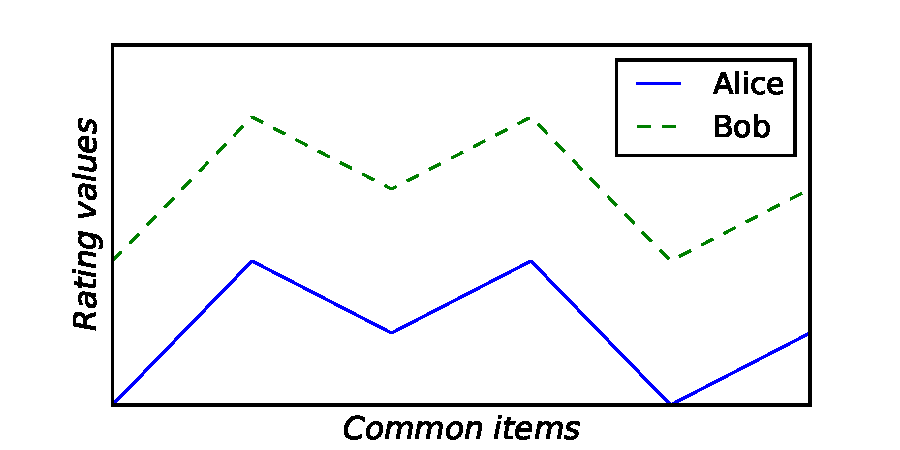
\includegraphics[width=4in]{figures/clones.pdf}
\caption{Bob is a perfect clone of Alice.}
\label{FIG_CLONES}
\end{figure}

It is obvious that in collaborative filtering, clones are of great interest when
it comes to predict a user's ratings, and yet the information they provide is
often discarded.  The principle underlying the analogical clone-based view is
the following: for predicting a missing rating for $u$ we not only look at its
nearest neighbors, but also to those $v$ whose rating are such that $r_{ui} =
r_{vi} + t_{vu}$ where $t_{vu}$ is a more or less constant \textit{correction
term} that can be either positive or negative.

In the next two sections, we investigate this idea of a clone-based prediction,
first when ratings are viewed as numerical quantities in section
\ref{NUMERICAL_POV}, and then when they have an ordinal meaning only in
section \ref{ORDINAL_POV}.

\subsection{Ratings as numerical quantities}
\label{NUMERICAL_POV}

In the following, we define $C_i(u)$ as the set of users that are clones of $u$
and that have rated item $i$.  From the previous definitions, one can easily
derive a very general collaborative filtering framework for predicting a user's
rating by taking into account its clones:
$$\predrui = \text{aggregation}(r_{vi} + t_{vu}), \quad \forall v \in
C_i(u),$$
where $t_{vu}$ is a \textit{correction term} that we need to add to $v$'s
ratings so that they correspond to those of $u$. We clearly have a
generalization of the $k$-NN approach, which we could write as:
$$\predrui = \text{aggregation}(r_{vi} + t_{vu}), \quad \forall v \in \{v \in C_i(u)
  | t_{vu} = 0\}.$$

Following this general framework, one can construct a great variety of
algorithms with various level of complexity. In the next subsections, we
propose a very straightforward algorithm, and a more efficient one.

\subsubsection{A straightforward prediction algorithm}
\label{STRAIGHTFORWARD}

In its most simple form, a user $v$ can be considered to be a $t$-clone of $u$ if
the ratings of $v$ differ from those of $u$ from a constant $t$:
\begin{equation}
v \in t\text{-}C(u) \iff \forall i \in I_{uv}, r_{ui} = r_{vi} + t.
\end{equation}
From then on, computing $\predrui$ amounts to finding all the users $v$ that
satisfy this criteria, and computing an aggregation of their rating for $i$,
which can simply be a mean. We implemented this basic algorithm described by
algorithm \ref{algo_straight}, and referred to as \textit{Bruteforce}.

 \begin{algorithm}[!ht]
   \caption{\textit{Bruteforce}}
       \label{algo_straight}
       \begin{algorithmic}

      \STATE {\bf Input}: A set of known ratings $R$, a user $u$, an item
      $i$ such that $r_{ui} \notin R$.
      \STATE {\bf Output}: $\hat{r}_{ui}$, an estimation of $r_{ui}$

      \STATE {\bf Init}:
      \STATE $C = \varnothing$ \quad \quad // list of candidate ratings
      \FORALL{ users $v \in U_i$}
        \FORALL{$t$}
          \IF{$v \in t\text{-Clones}(u)$}
          \STATE $C \gets C \cup \{r_{vi} + t\}$ \quad // add x as a candidate rating
          \ENDIF
        \ENDFOR
	    \ENDFOR
    \STATE $\hat{r}_{ui} = \aggr{x \in C} x$
\end{algorithmic}
\end{algorithm}

Of course, one may want to relax the definition of a $t$-clone, as the current
one is too strict and only very few users will satisfy this criteria. In our
implementation, we chose the following condition:
$$v \in t\text{-}C(u) \iff \sum_{i \in I_{uv}} |(r_{ui} - r_{vi}) - t| \leq |I_{uv}|.$$
This amounts to accept $v$ as a $t$-clone of $u$ if on average, $r_{ui} -
r_{vi}$ is equal to $t$ with a margin of $1$.

The values of $t$ clearly depend on the rating scale. The dataset on which we
tested our algorithms use the $[1, 5]$ interval, so possible values for $t$
that were considered are integer values between $[-4, 4]$.

This is obviously a very rough algorithm, to which one could point out numerous
flaws, but its purpose is to show that even such a basic clone-based approach
can lead to better results than a basic neighborhood method.

\subsubsection{Modeling clones with the similarity measure}
\label{MODELING_CLONES}
Another option to consider clones is to use the well known neighborhood-based
formula, and capture their effect inside an appropriate similarity measure. The
general neighborhood formula is as follows \cite{RecoSystemHandbook}:

$$\predrui = \frac{\sum_{v \in N_i^k(u)} r_{vi} \cdot sim(u, v)}{\sum_{v \in
  N_i^k(u)} sim(u, v)},$$
where $N_i^k(u)$ is the set of the $k$ nearest neighbors of $u$ that have rated
$i$. So, we move from a crisp view of the set of clones to a fuzzy one. In
fact, the above formula looks very similar to the interpolation principle
underlying Takagi-Sugeno fuzzy controller where similarity degree is viewed as
a fuzzy membership grade \cite{TakSug85}.

The above formula is commonly used with classical similarity metrics such as
Pearson or cosine similarity, or inverse of MSD (Mean Squared Difference, which is
a distance).
However, these similarities are not plainly satisfactory when it comes to
clones. Indeed with these metrics, two users are considered to be close if
their common ratings are often the same, but two perfect clones $u$ and $v$
with a significant correction term $t_{vu}$ would be considered as far from
each other, thus involving a loss of information.

A simple choice to measure how two users relate as clones can be the following:
$$Clone\_dist(u, v) =  \frac{1}{|I_{uv}|} \cdot \sum\limits_{i \in I_{uv}}
((r_{ui} - r_{vi}) - \mu_{uv})^2$$
where $\mu_{vu}$ is the mean difference between ratings of $u$ and $v$:
$$\mu_{uv}= \frac{1}{|I_{uv}|}\sum_{i \in I_{uv}} (r_{ui} - r_{vi}).$$

One can understand this distance in two ways:
\begin{itemize}
\item it can be regarded as the variance of the difference of ratings between
  $u$ and $v$,
\item or it can be regarded as a simple MSD measure ($\text{MSD}(u, v) =
  \frac{1}{|I_{uv}|} \cdot \sum\limits_{i \in I_{uv}}
  (r_{ui} - r_{vi})^2$)
 to which the mean difference of ratings between $u$ and $v$ has been
 subtracted.
  \end{itemize}

As our measure $Clone\_dist$ is a distance, it is necessary to transform it
into a similarity measure. Common choice is to take its inverse (while accounting for zero division): $Clone\_sim(u,
v) = \frac{1}{Clone\_dist(u, v) + 1}$.

Once we know how to find the clones of a user, it is a simple matter to output
a prediction using the classical neighborhood approach:
$$\predrui = \frac{\sum_{v \in N_i^k(u)} (r_{vi} + \mu_{uv}) \cdot sim\_clone(u,
v)}{\sum_{v \in N_i^k(u)} sim\_clone(u, v)}.$$

This algorithm will be referred to as $CloneA$. For the sake of completeness,
we also tried the same formula but with a more basic similarity metric that
does not care about clones: MSD. This algorithm is referred to as $CloneB$.

\subsubsection{ZOB}

A more sophisticated prediction, popularized by \cite{BelKorSIGKDD2007} is as
follows:
$$\predrui = b_{ui} + \aggr{v \in N_i^k(u)}(r_{vi} - b_{vi}),$$
where $b_{ui}$ is a baseline (or bias) related to user $u$ and item $i$. It
is supposed to model how $u$ tends to give higher (or lower) ratings than the
average of ratings $\mu$, as well as how $i$ tends to be rated higher or lower
than $\mu$. As it uses the neighbourhood of users to output a prediction, this
technique tends to model local relationships in the data.

Note that it is perfectly possible to proceed in an item-based way. Indeed,
rather than looking for users similar to $u$, one may look for items similar to
$i$, which leads to formulas dual of the above ones.


A simple and efficient formula using neighborhood technique, popularized by
\cite{KorACM2010} is the following:
$$\predrui = b_{ui} + \frac{\sum_{v \in N_i^k(u)} (r_{vi} - b_{vi}) \cdot
sim(u, v)} {\sum_{v \in N_i^k(u)}sim(u, v)}.$$
It is based on a simple $k$-NN approach, where are added the $b_{ui}$ terms,
called \textit{baselines}: $b_{ui} = \mu + b_u + b_i$. $\mu$ is the global mean
of all ratings in $R$. The $b_u$ term is intended to capture users propensity
to give ratings higher or lower than the global mean $\mu$, and the same goes
for items with $b_i$: some items tend to be rated higher than others. Baselines
are computed by solving a least squares problem:
$$ \min\limits_{b_u, b_i} \sum_{r_{ui} \in R} (r_{ui} - (\mu + b_u + b_i))^2,$$
which can be achieved efficiently by stochastic gradient descent, or
alternating least squares.

Among recommended similarity metrics, this one is of particular interest:
$$\text{sim}(u, v) = \frac
{ \sum\limits_{i \in I_{uv}} (r_{ui} -  b_{ui}) \cdot (r_{vi} - b_{vi})}
{\sqrt{\sum\limits_{i \in I_{uv}} (r_{ui} -  b_{ui})^2} \cdot
\sqrt{\sum\limits_{i \in I_{uv}} (r_{vi} -  b_{vi})^2}}.$$

It is simply a Pearson correlation coefficient, except that instead of
centering ratings by their means, they are centered with the baseline
predictors. An intuitive and illuminating way to look at this algorithm as a
whole is to see that it conceptually follows these steps:
\begin{enumerate}
  \item Compute $R'$, the set of all ratings normalized by the corresponding
    baseline: $r'_{ui} = r_{ui} - b_{ui}$.  $R'$ can be regarded as the set
    where all ratings are given from the same frame of reference, thus
    discarding any bias.  In $R'$, ratings can then be considered as absolute.
  \item Using $R'$, compute similarities between users using the cosine similarity (the
    cosine similarity is the same as the Pearson correlation coefficient,
    except that quantities are not centered).
  \item Output a prediction using the basic $k$-NN formula. As this prediction
    belongs to the same space of $R'$ where ratings have no bias, it needs to
    be transposed back to the space of $R$ (for performance evaluation
    purposes).
\end{enumerate}

In what follows, this algorithm is referred to as $k$-NNbsl.


It is very clear that the use of the baseline predictors is motivated by the
same reasons one would want to consider clones in a rating prediction
algorithms. This means that $k$-NNbsl implicitly takes the idea of clones into account, and thus a form of analogical reasoning.
Differences and resemblances of these two approaches are discussed
in the next section.

\subsubsection{Experiments and discussion}
\label{expeDiscuss}

We evaluated the performance of the aforementioned algorithms in terms of MAE
and RMSE on two datasets, the movielens-100K and movielens-1M
datasets\footnote{http://grouplens.org/datasets/movielens}, containing
$100,000$ and $1M$ ratings respectively. Results are shown in tables
\ref{table:res100k} and \ref{table:res1M} and where calculated using 5-folds
cross-validation. For each of these algorithms, the number of neighbors or
clones used to output a prediction is $k = 40$, except for the bruteforce
algorithm where the number of clones can not be controlled.
\begin{table}[!ht]
\centering
\caption{Performance of algorithms on the Movielens-100k dataset}
\label{table:res100k}
\begin{tabular}{| c || c | c | c | c | c | c |}
\toprule
     &  k-NN & Bruteforce & Clone A & Clone B & $k$-NNbsl\\
\midrule
RMSE & .9763 &   .9461    &   .9353 &  .9311  &  .9338   \\
MAE  & .7705 &   .8576    &   .7327 &  .7321  &  .7337   \\
\bottomrule
\end{tabular}
\end{table}

\begin{table}[!ht]
\centering
\caption{Performance of algorithms on the Movielens-1M dataset}
\label{table:res1M}
\begin{tabular}{| c || c | c | c | c | c | c |}
  \toprule
     &  k-NN & Bruteforce & Clone A & Clone B & $k$-NNbsl\\
  \midrule
RMSE & .9216 &           .&   .8996 &  .8969  &  .8879\\
MAE  & .7252 &           .&   .7057 &  .7050  &  .7005\\
\bottomrule
\end{tabular}
\end{table}

It is very clear that even a very straightforward approach of the clone-based
recommendation principle significantly outperforms the most basic $k$-NN
algorithm. It is however a lot heavier to compute, thus not very suitable for
real world recommendation purposes (its performances on the Movielens-1M
dataset simply could not be computed). The two other clone-based algorithms
however, have the exact same complexity of any $k$-NN-based algorithm which is
a significant improvement from the algorithm described in section
\ref{ANALOGY_USERS}.

Surprisingly enough, out of the two Clone algorithms, it is the one that does
not care about clones in its similarity measure that achieves the best results.
This might be due to the fact that in the neighborhood based on MSD, $\mu_{uv}$
is necessarily small and thus easier to estimate in a statistical significant
way.

Performances of the Clone algorithms are close to those of the state of the
art $k$-NNbsl algorithm. It is however important to understand that these
algorithms differ on the following points:
\begin{itemize}
\item The Clone algorithms do not address item bias, which is a significant
  drawback. It may not be unreasonable to believe that incorporating item bias
  in the prediction would lead to better results.
\item There is a subtle yet meaningful difference of interpretation between the
  biases induced by both algorithms. In the clone algorithm, biases are all
  pairwise, meaning that they involve two users, and they are computed on items
  that both users have rated. As for the $k$-NNbsl algorithm, there is no such
  thing as a pairwise bias. Bias for a given user is computed using only its
  own ratings, and is a result of a global optimization problem involving the
  global mean of all ratings, which means that every single rating in $R$ has
  an impact on the bias.
\item On the biggest dataset (Movielens-1M), the $k$-NNbsl algorithm appears to
  achieve better accuracy than the other algorithms, while this is not the case
  for the small dataset. A possible explanation is that as baselines are
  computed on the whole training set, they tend to capture most of the noise
  when the training set gets bigger, thus improving accuracy compared to more
  heuristic-based approach.
\end{itemize}

It should also be noted that in fact, it is recommended to perform a shrinkage
on the similarity measure of algorithm $k$-NNbsl, in order to take into account
the number of common items between two users: the more items they share, the
more confident we are when computing their similarity \cite{KorACM2010}. Such
an approach can improve significantly both RMSE and MAE of the algorithm.
Similarly, in the clone-based approach, it might be of interest to discount
clones that rely on a too small number of common items.

\subsection{Towards an ordinal view of ratings}
\label{ORDINAL_POV}

We may wonder if one can devise a counterpart of the numerical clone-based
approach, which would be compatible with an ordinal view of the ratings.
Indeed, an extreme way for unbiasing and comparing two sets of ratings is to
forget about their numerical values, and only consider their rankings.  The
idea of viewing ratings in a ordinal manner has been advocated in
\cite{KorSillRECSYS11}.
In this section, we discuss an ordinal counterpart of the analogical approach
previously presented.  Analogical reasoning with ordinal data has first been
proposed in \cite{MicBarCAP09}, yet with a different concern.

\subsubsection{An algorithm for rank prediction}
Indeed the idea that ``\textit{the rating of user $u$ for item $i$ is to the
rating of user $v$ for item $i$ as the rating of user $u$ for item $j$ is to
the rating of user $v$ for item $j$}’’ may be understood  as well in an ordinal
manner. This leads to state that ``\textit{the relative ranking of item $i$
  among the ratings given by user $u$  is to the relative ranking of item $i$
  among the ratings given by user $v$ as the relative ranking of item $j$ among
  the ratings given by user $u$  is to the relative ranking of item $j$ among
the ratings given by user $v$}.

This means that we need to compare the rankings given by two users $u$ and $v$
on their common items. In the following, $\rho_{ui}$ denotes the relative
ranking of item $i$ out of all the items rated by $u$. Our goal is to estimate
all values of $\rho_{ui}$, for any user and any item. The main steps of a
possible algorithm is as follows:
\begin{enumerate}
  \item Compute similarities between users, based on their rankings. A very
    popular similarity ranking measure is the Spearman's rank correlation
    coefficient, or Spearman's rho.
  \item Compute an estimated rank $\hat{\rho}_{ui}$ as an aggregation of all the
    rankings $\rho_{vi}$ extracted from the $k$ nearest neighbors (using
    Spearman's rho as similarity):
    $$\hat{\rho}_{ui} = \frac{\sum_{v \in N_i^k(u)} \rho_{vi} \cdot
    sim(u, v)}{\sum_{v \in N_i^k(u)} sim(u, v)}.$$
\end{enumerate}

This is obviously very similar to the neighborhood approach described in
section \ref{MODELING_CLONES}, but instead of predicting a rating, we output a
predicted rank. This approach is denoted as \textit{RankAnlg}.


\subsubsection{Experiments}

We evaluated the performance of our algorithm and compared it to other
previously described approaches, using the exact same evaluation protocol as in
section \ref{expeDiscuss}. The Movielens-1m dataset was not benchmarked, as our
algorithm is too computationally intensive.

RMSE and MAE are good measure for evaluation rating prediction accuracy, but
are not suitable when it comes to evaluate rankings. A better measure is the
Fraction of Concordant Pair, which evaluates the probability that given any two
items $i$ and $j$ rated by any user $u$, the system has correctly estimated
whether $u$ prefers $i$ over $j$ or the inverse. To compute the FCP, we need to
intermediate measures. $c_u$ defines the number of concordant pairs for user
$u$, and $d_u$ its number of discordant pairs. The FCP is then computed over all
users as the proportion of concordant pairs.

\begin{align*}
&c_u = \{(i, j) \in I^2 \quad s.t. \quad \predrui > \predruj \text{ and }
r_{ui} > r_{uj}\}\\
&d_u = \{(i, j) \in I^2 \quad s.t. \quad \predrui \geq \predruj \text{ and }
r_{ui} < r_{uj}\}\\
&FCP = \frac{\sum\limits_{u \in U} c_u}{\sum\limits_{u \in U} c_u + \sum\limits_{u \in U} d_u}
\end{align*}
Note that $\predrui$ here may represent either a rating prediction or a
ranking prediction $\hat{\rho_{ui}}$.

Results are reported in table \ref{table:res100kRank}.

\begin{table}[!ht]
\centering
\caption{Performance of algorithms on the Movielens-100k dataset (ranking
evaluation)}
\label{table:res100kRank}
\begin{tabular}{| c || c | c | c |}
\toprule
     & RankAnlg &  k-NN & $k$-NNbsl\\
\midrule
FCP  &  .7063   & .7096 &  .7163   \\
\bottomrule
\end{tabular}
\end{table}

Unfortunately, even a basic algorithm that was not designed for ranking
prediction performs better in terms of FCP. To explain this difference, one may
look at the distribution of average support over all the predictions, as shown
on figure \ref{FIG_SUPPORT}. Between
two users $u$ and $v$, the support is defined as the number of common items
($|I_{uv}|$), which was used to compute the similarity between $u$ and $v$. For
a given prediction $\predrui$, the average support is the average of all the
supports $|I_{uv}|$ over all users $v \in N_i^k(u)$.

\begin{figure}[!h]
\centering
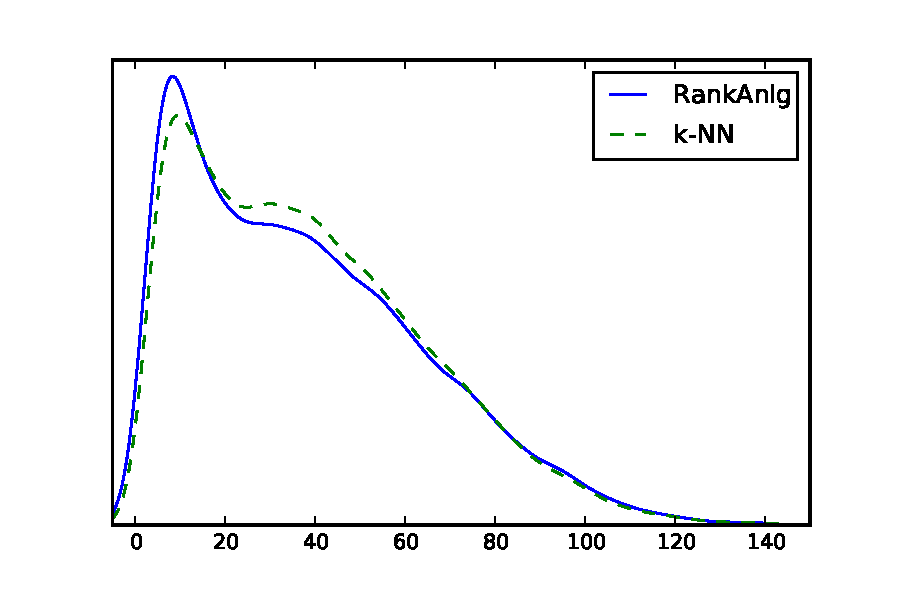
\includegraphics[width=2.5in]{figures/support.pdf}
\caption{Distribution of average support.}
\label{FIG_SUPPORT}
\end{figure}

The use Spearman's rho tends to provide with neighbors that have smaller
support, thus leading to a less significant and less accurate estimation of the
neighborhood, which may explain the differences in performance.

\section{Mining analogical proportions}

\subsection{Règles d'association}
Les règles d'association sont des informations extraites d'une base de
données qui révèlent des dépendances entre produits (aussi appelés
items).  Par exemple, partant
de la règle d'association $a \rightarrow b$  (si on achète $a$ alors il y a
de grandes chances que l'on achète $b$), un système de recommandation peut
suggérer $b$ dès lors qu'on a acheté $a$ mais pas encore $b$.  On définit
une règle d'association comme suit:

Soit $I= \{i_1,i_2,...,i_m \}$ un ensemble d'items. Soit $T= \{t_1, t_2,...,t_n
\}$ un (multi)-ensemble de transactions, i.e.,  $t_i \subseteq  I$. Une règle
d'association s'exprime sous la forme $X \rightarrow Y$ o\`u $X \subset I ,~ Y
\subset I, $ et $X \cap Y = \emptyset$.  $X$ et $Y$ sont des ensembles d'items
(appelés par la suite \textit{itemsets}), et le \emph{support} $supp(X)$ d'un
itemset $X$ est défini comme la proportion de
transactions qui le contiennent.  Un certain nombre de mesures permettent
d'\'evaluer la {\it qualité} d'une règle d'association, comme  la
\emph{confiance} qui s'exprime sous la forme $\frac{supp( X \cup Y)}{supp(X)}$.

Les méthodes d'extraction de telles règles ont fait l'objet de nombreuses
études. L'algorithme {\it Apriori}
\cite{AgrSriVLDB94} est probablement le plus connu mais il en existe d'autres.
L'idée   est de fixer un seuil minimum $\alpha$ pour le support et de chercher dans
$2^I$ les itemsets dont le support dépasse $\alpha$, pour obtenir un ensemble
$S$ d'itemsets fréquents. Cette recherche est facilitée par le fait que
tout sous-ensemble d'un itemset fréquent est aussi fréquent.

On se fixe alors un nouveau seuil $\beta$ pour la confiance.  Dès lors que
l'on dispose d'un itemset $IS$ de $S$, on peut chercher toutes les partitions
de $IS$ sous la forme $X \cup Y = IS$, calculer la confiance de la règle $X
\rightarrow Y$, ne garder cette règle que si sa confiance dépasse le seuil
$\beta$.

L'algorithme retourne finalement un ensemble de règles d'association
respectant les critères de qualité exigés, et fournissant donc un certain
nombre d'informations sur les liens entre les éléments de la base de
données.
%Sur le mode des proportions analogiques, on admettra que {\it le dentifrice
%est à la brosse à dent ce que le beurre est à la biscotte}.  Dans ce
%cas, on peut penser recommander à quelqu'un ayant acheté dentifrice,
%brosse à dent et beurre, d'acheter des biscottes. Sur quelle base?  Sur la
%base que la relation liant dentifrice et brosse à dent est la même que
%celle liant beurre et biscottes.
Au même titre que les règles d'association, la détection de proportions
analogiques dans une base de données est une information supplémentaire
fournie aux détenteurs de la base.  Dans la section suivante, nous
utilisons l'algorithme {\it Apriori} pour extraire d'une base des proportions
analogiques.

\subsection{Trouver des analogies}
Dans la suite, on recherche des analogies dans une base de données dédiée à la
recommandation.
L'objectif d'un système de recommandation est de fournir à un utilisateur une
liste personnalisée d'articles susceptibles de l'intéresser.  Soit $U$ un
ensemble d'utilisateurs et $I$ un ensemble d'items. Pour certaines paires $(u,
i) \in U \times I$, on connait la note $r_{ui}$, qui exprime l'intérêt que
l'utilisateur $u$ porte à l'item $i$ : on trouvera souvent $r_{ui} \in
[\text{aime, n'aime pas}]$ ou bien $r_{ui} \in [1, 2, 3, 4, 5]$. Nous dénotons l'ensemble des notes
connues du système par $R$.
% Pour recommander des articles aux utilisateurs, un
%système de recommandation procède ainsi: i) avec un algorithme $A$, on estime
%les notes $r_{ui}$ inconnues (c.à.d.  $r_{ui} \notin R$);
%Cette estimation  $A(u, i)$ est communément notée $\hat{r}_{ui}$.
%ii) Avec une stratégie de recommandation $S$ et au vu des notes précédemment
%estimées, recommander des items aux utilisateurs.
%Par exemple, une stratégie très basique mais assez courante est de suggérer à
%$u$ les articles $i$ pour lesquels $\hat{r}_{ui}$ est le plus grand.


Notre approche s'applique donc au cas o\`u peu de notes sont connues.  Considérons
4 items  $A, B, C$ et $D$ pour lesquels on cherche à savoir s'ils constituent
une analogie valide, sans avoir pour l'instant d'idée sur l'ordre dans lequel
on doit les considérer. Comme pour les règles d'association, la notion de
support demeure puisque ces 4 items constituent un 4-itemset.  Par
définition:

%\small
$Supp(\{A, B, C, D \})= \frac{|U_{ABCD}|}{|U|}$, où $U_{ABCD}$ est l'ensemble
des utilisateurs qui ont conjointement noté $A, B, C,$ et $D$.

%Dans le cas d'une base de données de films comme MovieLens, le support de 4
%films $\{a, b, c, d \}$ est simplement la proportion d'utilisateurs ayant vu
%ces 4 films.
Naturellement, comme pour les règles d'association, on peut ne
s'intéresser qu'aux analogies dont le support est supérieur à un certain
seuil $\alpha$.  Ensuite, pour un itemset $\{A, B, C, D \}$ de support
supérieur au seuil $\alpha$ que l'on s'est fixé, et ayant à notre
disposition une relation analogique permettant d'affirmer si, par exemple,
$A:B::C:D$ est valide ou non, on cherche quelles sont les analogies possibles.

On sait qu'il y a 4! = 24 permutations possibles de $\{A, B, C, D \}$,
correspondant à 24 analogies possibles. Cependant, compte tenu des
propriétés de l'analogie, un certain nombre d'entre elles sont
équivalentes et mènent à 3 classes de 8 analogies équivalentes
représentées par:
\begin{itemize}
\item $A:B::C:D$
\item $A:B::D:C$
\item $A:D::C:B$
\end{itemize}
Il convient donc de ne chercher que ces trois classes d'analogies.  Pour ce
faire, on pourra se donner une fonction $f$ évaluant la qualité d'une
analogie, un autre seuil de qualité $\beta$, et ne retenir, parmi les trois
options possibles que celles dont la qualité dépasse le seuil $\beta$. Ce que
nous appelons la qualité ici joue le rôle de la confiance pour les règles
d'association.  En clair $A:B::C:D$ est retenue comme analogie  valide si et
seulement si $f(A:B::C:D) \geq \beta$.  A la fin de cette procédure, on obtient
donc un ensemble d'analogies qui représentent des relations entre quatre items.

\subsubsection{Exemples de fonction de qualité}
Tous les 4-itemsets considérés $A, B, C, D$ sont représentés par
des vecteur de notes.  La dimension de ces vecteurs est égale au nombre
d'utilisateurs ayant noté les quatre items.  Cela nous donne plusieurs options
pour mesurer la qualité d'une proportion $A:B::C:D$, qui dépend de la nature
des analogies considérées et donc implicitement de l'échelle de notes.

Dans le cas d'une échelle binaire ($r_{ui} \in [\text{aime, n'aime pas}]$), on
pourra choisir pour $f$ la proportion de composantes pour lesquelles l'analogie
tient parfaitement.  Si l'échelle est numérique, on dispose de plusieurs
techniques pour évaluer l'exactitude d'une proportion entre quatre réels, qui
donneront des valeurs entre 0 et 1. Là aussi, on peut envisager une
aggrégation de ces valeurs de vérité.  Toujours si l'échelle est réelle et en
utilisant la proportion arithmétique, on sait que $A, B, C, D$ forment un
parallèlogramme ssi l'analogie est parfaite. La qualité d'une analogie
$A:B::C:D$ est donc inversement proportionnelle à la déformation du
parallélogramme dans $\mathbb{R}^n$, que l'on peut calculer en termes de
distance euclidienne.  Enfin, en adoptant un point de vue statistique on peut aussi
s'intéresser à la probabilité d'observer $A:B::C:D$, et considérer que la
proportion est crédible si elle a peu de chance d'être dûe au hasard (voir
Section \ref{expe}).

\subsubsection{Algorithme}
L'algorithme d'extraction de règles analogiques est alors calqué sur le modèle
d'extraction de règles d'association : on se donne une fonction de qualité $f$,
et deux seuils $\alpha$ et $\beta$.

D'abord, on calcule tous les 4-itemsets de support supérieur au seuil $\alpha$
à   l'aide de l'algorithme \textit{Apriori}.  Pour chaque itemset retenu,
on calcule la qualité des trois formes possibles non équivalentes d'analogie, et on garde celles dont
la qualité dépasse le seuil $\beta$.

\begin{enumerate}
\item Entrée: une relation d'analogie, une fonction de qualité $f$, deux seuils
  $\alpha$ et $\beta$.
\item Calculer tous les 4-itemsets de support supérieur au seuil $\alpha$ à
  l'aide l'algorithm \textit{Apriori}.
\item Pour chaque itemset retenu, calculer, parmi les 3 formes possibles non
  équivalentes d'analogie, celles dont la qualité dépasse le seuil $\beta$.
\item Sortie : la liste des règles analogiques retenues.
\end{enumerate}

\subsection{Premières expériences}

Nous avons expérimenté cet algorithme sur la base de données
Movielens\footnote{http://grouplens.org/datasets/movielens/},
constituée de $100~000$ notes de $1700$ films par $1000$ utilisateurs. Chaque
note appartient à l'échelle $[1, 2, 3, 4, 5]$, mais nous l'avons ramenée à une
échelle binaire de la façon suivante : un utilisateur $u$ aime un film s'il lui
a attribué une note supérieure à $\mu_u$, où $\mu_u$ est la note moyenne que
$u$ donne aux films qu'il a vus.

En plus de choisir un critère de support minimal, nous avons aussi imposé un
support maximal : les films très populaires vus par beaucoup de monde font
généralement consensus (les gens les apprécient), et ont peu de chance de
construire des analogies intéressantes. Cela a de plus l'avantage de réduire
l'espace de recherche, et donc accélerer significativement la recherche de
4-itemsets. De plus, toujours dans le but d'éviter de construire des analogies
trop triviales, on ne retient pas les proportions de la forme $x:x::x:x$.

En choisissant un support minimal de 40 et un support maximal de 150, nous
obtenons les mesures de qualités (calculées comme la proportion d'analogies
parfaites) illustrées par la figure \ref{qualite}. Comme on peut le voir, la
meilleure proportion a une qualité d'environ $40$\%, ce qui peut paraître peu
convainquant. Néanmoins, en remarquant que pour une composante il y a 4 chances
sur 16 d'obtenir une analogie significative (on ignore les $x:x::x:x$), et en supposant que les composantes sont
indépendantes les unes des autres, le nombre de composantes pour lesquelles
l'analogie est vraie suit une loi binomiale de paramètres $\mathcal{B}(40,
\frac{1}{4})$, où $40$ est la dimension des vecteurs. Sous ces hypothèses, la
probabilité d'obtenir $40$\% ou plus d'analogies parfaites est de $0.026$, ce qui
tend à montrer qu'un tel quadruplet d'items reste significatif, en cela que la
proportion analogique observée a peu de chance d'être due au hasard.

\begin{figure}[h]
  \vspace{-0.4cm}
\caption{Qualité des proportions trouvées}
\label{qualite}
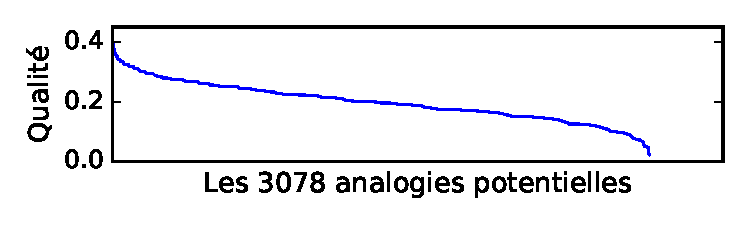
\includegraphics[scale=0.6]{figures/quality_of_proportions.pdf}
\vspace{-0.4cm}
\end{figure}
Les mêmes expériences ont été menées en gardant l'échelle de notes numérique
($[1, 2, 3, 4, 5]$) et en utilisant une expression multivaluée de l'analogie.
Les meilleures proportions obtenues s'avèrent être globalement les mêmes que
celles qui ressortent de l'échelle binaire, montrant ainsi la cohérence des
deux approches. La m\'ediocre qualit\'e des proportions analogiques trouv\'ees,
m\^eme si elles sont statistiquement significatives,
ne permet pas d'utiliser raisonnablement l'inf\'erence analogique dans cet exemple.
Ceci  tend \`a expliquer a posteriori pourquoi une approche pour la
pr\'ediction de notes manquantes, bas\'ee sur la recherche de triplets
analogiques, avait obtenu des r\'esultats modestes \cite{HugPraRicISMIS15}.
